\section{Background and Scope}
\label{sec:background}

\paragraph{E-graphs and equality saturation.}
An \emph{e-node} stores an operator and references to child \emph{e-classes},
where each e-class groups expressions already known to be equal~\cite{ogEgraphs1,egraphsOG,egg}.
For example, given $a\times 2=a+a$ and singleton classes $c_a=\{a\}$ and
$c_2=\{2\}$, a single class $c=\{\times(c_a,c_2),\;+(c_a,c_a)\}$ shares both
forms, and a parent $g(c)$ compactly represents both $g(a\times 2)$ and
$g(a+a)$ (Figure~\ref{fig:typed-slotted-egraphs}(a)).
% Preamble: \usepackage{graphicx,amsmath,amssymb}
% Place typed-slotted-egraphs.pdf beside the main LaTeX source.
\begin{figure}[t]
  \centering
  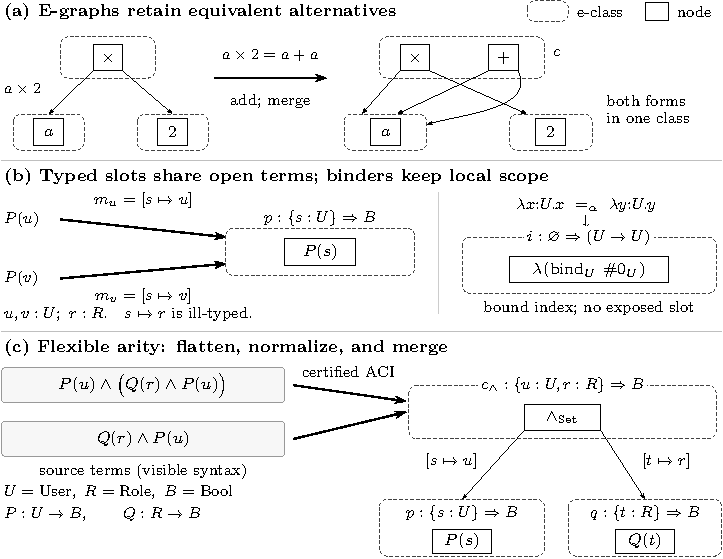
\includegraphics[width=\linewidth]{figures/typed-slotted-egraph-figure.pdf}
  \caption{E-graphs, typed slots, and flexible arity.
  (a) Rewriting retains equivalent alternatives.
  (b) Typed maps share shapes without equating distinct free invocations;
  bound indices stay local.
  (c) Certified associativity flattens visible syntax; the Set quotient removes
  order and duplicates. Dashed boxes are e-classes; solid inner boxes are e-nodes.}
  \label{fig:typed-slotted-egraphs}
\end{figure}

Propagating child merges to parents is \emph{congruence}. After union--find
merges classes, \emph{rebuilding} restores hash-cons invariants and propagates
new parent congruences. Equality saturation alternates rewriting and rebuilding
until saturation or a resource bound, and extraction picks a term under a cost
model. Our focus is how e-node keys and equality certificates combine algebraic
containers with typed open-term interfaces.

\paragraph{Algebraic structure.}
Associativity, commutativity, and idempotence play distinct roles. For
conjunction, associativity flattens nested binary nodes, commutativity ignores
operand order, and idempotence drops duplicates. Sequences preserve order and
multiplicity, bags preserve multiplicity only, and sets preserve neither. Flat
bags and sets avoid combinatorial blowup in AC rewriting~\cite{conchon2012canonized,kapur2021ModularAC}:
over $n$ distinct generators, complete binary AC closure creates $2^n-1$
nonempty subproduct classes and $3^n+1-2^{n+1}$ ordered binary nodes
(Appendix~\ref{app:formal-details}). Relational fixpoint engines such as
egglog~\cite{egglog,egglog_software} and E-graphs Modulo
Theories~\cite{zucker2025omeletsneedonionsegraphs} connect e-graphs with
canonical algebraic values; here we study how container quotients interact with
typed variable bindings.

\paragraph{Binding and typed slots.}
Renaming bound variables yields $\alpha$-equivalence, as in
$\forall x{:}T.\,P(x)$ and $\forall y{:}T.\,P(y)$
(Figure~\ref{fig:typed-slotted-egraphs}(b)). When sharing an open body $P(x)$
across contexts, each occurrence must record which caller variable supplies $x$.
Slotted e-graphs~\cite{slottedEGraphs} attach a finite slot interface $S_a$ to
each class $a$ and write an occurrence as $m*a$, where $m$ maps $S_a$ into the
caller context. In our typed setting, a \texttt{User} slot maps only to a
\texttt{User} coordinate and a \texttt{Photo} slot only to a \texttt{Photo}
coordinate, while distinct variables of the same sort remain distinct slots.
Related approaches represent open terms functionally~\cite{zucker2026lifting} or
via hierarchical hypergraphs~\cite{egBindings}. We use de Bruijn
indices~\cite{deBruijn,maziarz2021HashingAlpha} for local bound positions and
typed slots for free positions. A binder-block descriptor records types,
domains, multiplicities, disjointness, and dependencies so that only
semantically justified block permutations enter the structural relation.

\paragraph{Alloy and bounded checking.}
Alloy~\cite{alloy,kodkod} models relational structures and temporal formulas
over signatures and fields. In the social-media model used in our running
example (Figure~\ref{fig:alloy-certificate-example}), \texttt{User} and
\texttt{Photo} are signatures, \texttt{Ad} extends \texttt{Photo}, and fields
such as \texttt{follows: set User} and \texttt{sees: set Photo} declare binary
relations. Relational join (\texttt{u.follows.posts}) composes relations,
membership (\texttt{p in u.sees}) tests containment, and quantifiers
(\texttt{all u: User | ...}) range over typed sets. The Alloy Analyzer checks
formulas within finite object scopes and trace bounds. In our Alloy4Fun
corpus~\cite{alloy4funDataset2023,alloy4fun,novice}, student submissions are
labeled relative to an oracle: \texttt{CORRECT}, overconstrained (excluding
valid instances), underconstrained (admitting invalid instances), or both.

\paragraph{Formal vs.\ empirical scope.}
Throughout the paper, we separate three kinds of claims:
(1)~\emph{formal-model theorems} proved in Lean~4.33.0 about abstract typed
slotted presentations, realizers, and certificate-preserving graph traces;
(2)~\emph{implementation checks} executed on the Java system (in-process strict
transition invariants, standalone certificate-verifier tests, bounded Alloy
counterexample searches, and native-operation replay audits); and
(3)~\emph{empirical observations} measured on natural, controlled, and synthetic
workloads. Observed agreement between two Java implementations is an empirical
check on those runs, not a universal equivalence proof, and end-to-end formal
refinement from Alloy source through the Java parser to Lean remains open.
